\chapter{Diseño e implementación} % Main chapter title

\label{Chapter3} % Change X to a consecutive number; for referencing this chapter elsewhere, use \ref{ChapterX}


En este capítulo se describe cómo se han utilizado las herramientas mencionadas en el capítulo \ref{Chapter2} y sus integraciones. Se presenta la arquitectura de alto nivel completa y luego se describe detalladamente desde el consumo de datos hasta la salida del proceso y su almacenamiento.


\section{Arquitectura del sistema}

En la figura \ref{fig:arqsistema} se puede observar la arquitectura de alto nivel que integra las herramientas utilizadas en la fase de entrenamiento y evaluación de los modelos de IA con las herramientas utilizadas para el despliegue.

\begin{figure}[htbp]
	\centering
	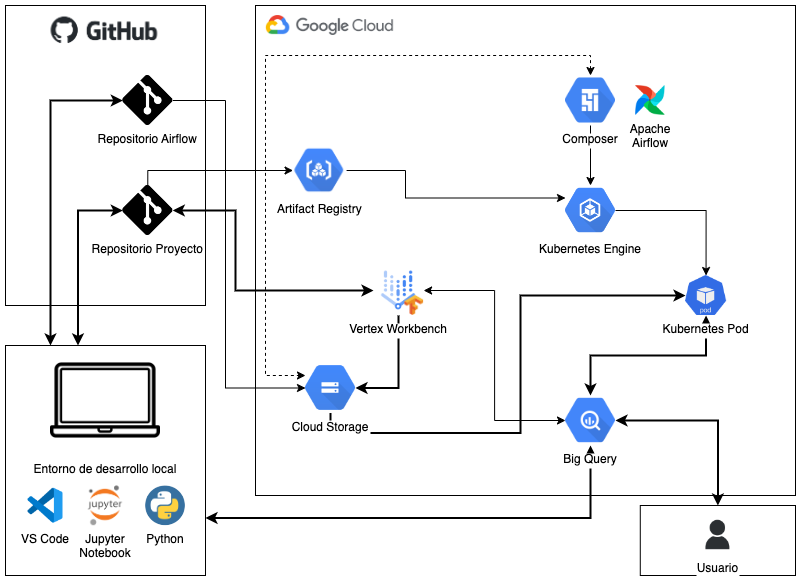
\includegraphics[width=1\textwidth]{./Figures/arq-sistema.png}
	\caption{Diagrama de la arquitectura de alto nivel.}
	\label{fig:arqsistema}
\end{figure}

La mayor parte del desarrollo se realizó en una computadora local, que contaba con un intérprete de Python y Visual Studio Code con Jupyter para la escritura de código. Estos archivos se sincronizaban contra un repositorio de GitHub.

Los datos para realizar el entrenamiento de los modelos de IA fueron tomados del \textit{data warehouse} BigQuery utilizando consultas SQL y bibliotecas de Google para Python para manejar su ejecución.

Estos datos son llevados a BigQuery por un proceso ajeno a este desarrollo, que se encarga de sincronizar la base de Salesforce hacia el \textit{data warehouse} diariamente. Particularmente, hay una tabla que contiene los reclamos y consultas de los usuarios, con su identificador de caso, fecha de creación y estado.

En las ocasiones en las que fue necesario un mayor poder de cómputo a través del uso de una placa de vídeo dedicada, se utilizó una instancia de Vertex AI Workbench en la nube de Google. Por lo general, estas situaciones se dieron al momento de realizar distintas pruebas con las redes neuronales BERT. Los modelos eran luego exportados al almacenamiento de la nube llamado Cloud Storage en formato ``Pickle'' o ``HDF5'' \textit{(Hierarchical Data Format 5)}.

El repositorio del proyecto cuenta con un Workflow de GitHub Action que se corre manualmente y genera una imagen de Docker, incluyendo bibliotecas y librerías necesarias, archivos de código y de configuración. Esta imagen de Docker es enviada al Artifact Registry de la nube de Google y almacenada allí.

Por otro lado, se trabajó en otro repositorio separado, que es único para manejar todos los flujos de trabajo de Apache Airflow que tiene el área de \textit{machine learning}. Este repositorio es exclusivo para la etapa de despliegue, y se agregó el DAG que administra el proceso de predicción.

El repositorio de Airflow cuenta con un Workflow de GitHub Action que sincroniza el código de los DAGs contra un Cloud Storage que está conectado a la instancia del orquestador. Airflow periódicamente controla si hay un flujo de trabajo nuevo y cuando lo detecta, lo carga.

Al momento de ejecutar el proceso, Airflow utiliza un operador dentro del DAG para conectarse con la plataforma de Kubernetes en instancia un Pod. Este Pod ejecuta los archivos de código del contenedor que se empaquetaron en la imagen de Docker cargada previamente en el Artifact Registry.

Al finalizar, se guardan los resultados de las predicciones en una tabla en BigQuery y el Pod es eliminado de Kubernetes. Los datos quedan disponibles en la base para que cualquier usuario con los suficientes permisos pueda consumirlos ejecutando una consulta a la base.

\section{Extracción y preprocesamiento del texto}

En esta sección se describen en detalle los pasos realizados para obtener los datos crudos y aplicarles un preprocesamiento para poder usarlos de entrada en el posterior entrenamiento de los modelos de IA.

\subsection{Extracción de datos de BigQuery}

Inicialmente se realizó un relevamiento de las tablas existentes, y en particular se encontró una tabla que contenía información de los reclamos y consultas. 

Las columnas de interés de esa tabla fueron:
\begin{itemize}
	\item El identificador del caso.
	\item El número del caso.
	\item La categoría L2 (de segundo nivel).
	\item La categoría L3 (de tercer nivel).
	\item El estado del caso.
	\item La descripción: el contenido del mensaje que escribió el usuario.
	\item La fecha de creación.
	\item La fecha de cierre.
\end{itemize}

Para la fase de entrenamiento, se limitó la extracción de casos a los que tenían fecha de creación entre enero de 2021 y diciembre de 2022. Además, su estado debía ser ``Resuelto'' o ``Cerrado''. Sin embargo, por la poca cantidad de datos que había para algunos clasificadores L2, fue necesario realizar consultas adicionales para tomar casos de 2023. Una vez obtenidos los datos, se guardaron en archivos ``Parquet'' para su posterior uso con la librería Pandas para Python.

Por otro lado, el área de atención al cliente maneja un archivo CSV \textit{(comma-separated values)} con la jerarquía de casos L1, L2 y L3. Es decir, para cada L1, qué casos L2 le corresponden, y para cada uno de esos L2, qué casos L3 le corresponden. Las categorías L3 fueron ignoradas para este trabajo, por lo que se hará foco en las primeras dos.

En total, se encontraron 15 categorías L1 y 122 categorías L2. Luego de una reunión con el área de atención al cliente para un mejor entendimiento de cada una, se descartó una categoría especial. Luego de este refinamiento quedaron 14 L1 y 117 L2.

En la figura \ref{fig:catl2porl1} se puede observar para cada categoría L1 cuántas subcategorías L2 contiene.

\begin{figure}[htbp]
	\centering
	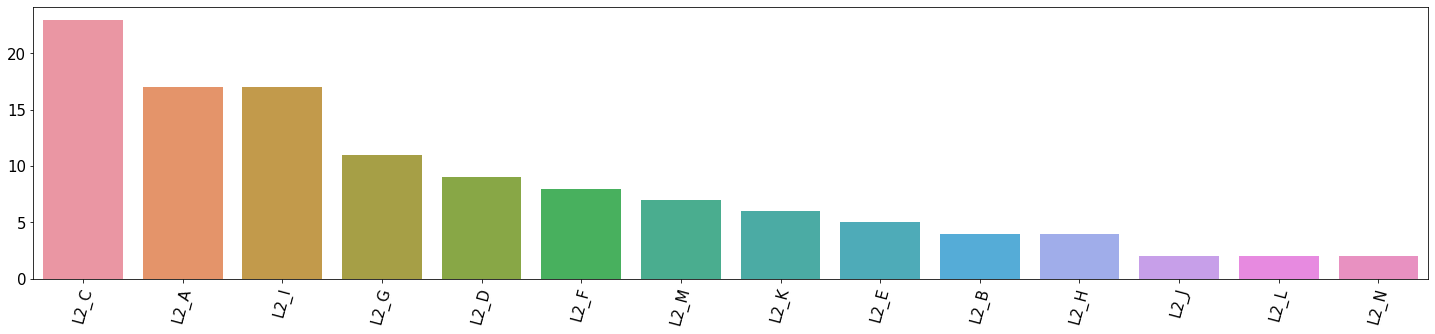
\includegraphics[width=1\textwidth]{./Figures/catl2porl1.png}
	\caption{Cantidad de categorías L2 para cada L1.}
	\label{fig:catl2porl1}
\end{figure}

Para trabajar en la fase de preprocesamiento, se combinó el archivo de los casos con el archivo que contenía la jerarquía de categorías, obteniendo así la L1 de cada reclamo y consulta.

\subsection{\textit{Pipeline} de preprocesamiento}

El preprocesamiento es una de las tareas más importantes en PNL. Los datos en crudo pueden contener información que no es relevante para la tarea en cuestión, que se debe eliminar. Por otro lado, muchos modelos de IA requieren un formateo previo de los datos para poder consumirlos.

En la figura \ref{fig:pipeline-texto} se detallan los pasos realizados para ``limpiar'' el texto.

\begin{figure}[htbp]
	\centering
	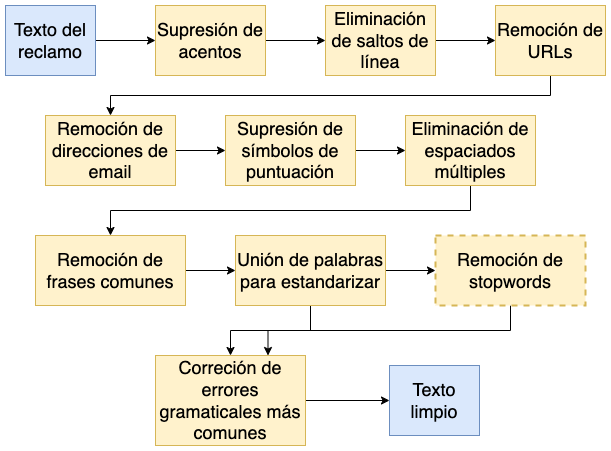
\includegraphics[width=.7\textwidth]{./Figures/pipeline-texto.png}
	\caption{Diagrama del procesamiento del texto crudo.}
	\label{fig:pipeline-texto}
\end{figure}

El proceso comienza con el texto original del reclamo tal cual quedó guardado en la base. Luego se le aplican las siguientes acciones:
\begin{enumerate}
	\item Se suprimen los acentos de las palabras (si los hubiera) utilizando una expresión regular.
	\item Se eliminan los saltos de línea.
	\item Se sacan URLs en el mesaje en caso de que hubiese hipervínculos.
	\item Se sacan direcciones de \textit{email}. Estos por lo general aparecen cuando el reclamo se hace a través de ese medio.
	\item Se suprimen signos de puntuación utilizando otra expresión regular.
	\item Se eliminan espacios múltiples para normalizar en un espacio entre dos palabras.
	\item Se remueven frases que se repiten en muchos reclamos: algunos casos quedan registrados en la base con la respuesta por parte de la empresa. Estos mensajes tienen una plantilla de base con frases que luego se repiten entre casos.
	\item Se unen palabras con un significado específico: por ejemplo ``pedidos ya'' se deja como ``pedidosya'' porque hace referencia a una empresa.
	\item Para el caso de los modelos de CNB entrenados, se aplicó un paso extra para eliminar \textit{stopwords}.
	\item Por último se realizó un análisis con los datos de entrenamiento para ver los errores gramaticales más comunes utilizando la librería PyEnchant para Python. De esto se obtuvo un listado con los errores más comunes y un mapeo a su versión correcta. En este paso se aplica la corrección sobre ese listado de palabras.
\end{enumerate}

Una vez obtenido el texto limpio, se procede a pasarlo a un vector numérico para que sea intepretado por los modelos de IA. Se distinguen dos formas de hacerlo, dependiendo de si se usa el modelo de CNB o el de BERT.

\subsubsection{Codificación para CNB}

En la figura \ref{fig:pipeline-baseline} se explica el proceso para obtener los vectores numéricos para entrenar el modelo de CNB. Al texto limpio se le aplica un paso de segmentación para obtener los \textit{tokens} que luego serán vectorizados utilizando el método TF-IDF. Por otro lado, a la variable objetivo que también esta en formato de texto, se le aplica el proceso de \textit{label encoding} para obtener una variable numérica. 

\begin{figure}[htbp]
	\centering
	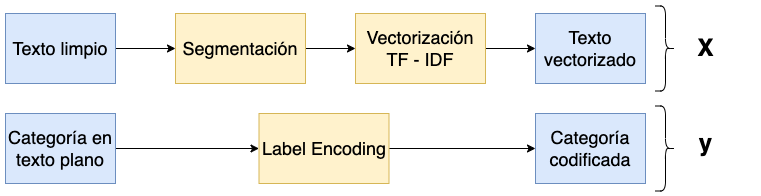
\includegraphics[width=.7\textwidth]{./Figures/pipeline-baseline.png}
	\caption{Diagrama de codificación para CNB.}
	\label{fig:pipeline-baseline}
\end{figure}

\subsubsection{Codificación para BERT}

En la figura \ref{fig:pipeline-bert} se puede ver el proceso para el caso de BERT. Se puede notar que es un poco mas largo que el de CNB.

\begin{figure}[htbp]
	\centering
	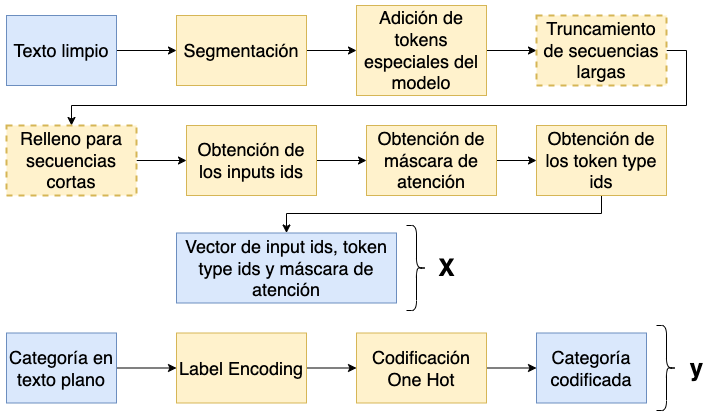
\includegraphics[width=.7\textwidth]{./Figures/pipeline-bert.png}
	\caption{Diagrama de codificación para BERT.}
	\label{fig:pipeline-bert}
\end{figure}

El algoritmo de segmentación de BERT se llama \textit{WordPiece} y tiene la particularidad de que no sólo segmenta por palabras sino que también lo hace por subpalabras y por caracteres. Arranca segmentando por todos los caracteres del vocabulario con el que fue entrenado y luego los va uniendo en pares. 

Utiliza la siguiente fórmula para computar los puntajes de los pares de \textit{tokens} a unir:
\begin{equation}
puntaje = \frac{\text{frecuencia del par}}{\text{frecuencia del primer elemento}\times \text{frecuencia del segundo elemento}}
\end{equation}
Luego une los pares con mayor puntaje y re-calcula para todos los \textit{tokens} resultantes. Este proceso es repetido hasta alcanzar un umbral para el puntaje o hasta alcanzar un límite de \textit{tokens}.

El vocabulario del modelo pre-entrenado de BERT que se utilizó está compuesto por 977 \textit{tokens} reservados del estilo ``[MASK]'' o ``[PAD]'' por ejemplo y luego por \textit{tokens} de caracteres individuales, subpalabras y palabras. \citep{WEBSITE:22}

En la figura \ref{fig:segmentacion-bert} podemos ver un ejemplo de cómo es segmentada una oración.

\begin{figure}[htbp]
	\centering
	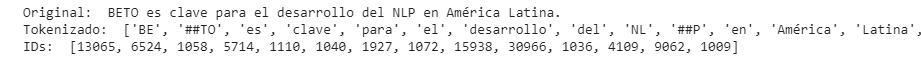
\includegraphics[width=1\textwidth]{./Figures/cap3-segmentacion.png}
	\caption{Ejemplo de segmentación \textit{WordPiece}\protect\footnotemark.}
	\label{fig:segmentacion-bert}
\end{figure}

\footnotetext{Imagen tomada de \url{https://espejel.substack.com/p/beto-bert-01-importacion-y-tokenizing}}

Luego de hacer la segmentación de cada frase, se hace un truncamiento de las secuencias largas a un máximo preestablecido y se realiza un relleno a las secuencias cortas con un \textit{token} especial hasta ocupar ese mismo máximo.

Los siguientes pasos son obtener los \textit{input ids} que son los identificadores de los \textit{tokens}, obtener la máscara de atención que marca qué \textit{tokens} la red debe mirar y por último obtener los \textit{token type ids} que marcan a qué secuencia pertenece cada \textit{token} (recordar que BERT se entrena de a pares de secuencia).

Por otro lado, la codificación de la variable objetivo es igual que en CNB solo que a la variable numérica obtenida se le aplica una codificación \textit{one hot} adicional.

\section{Entrenamiento de los modelos}

En esta sección se describe en detalle: los análisis exploratorios realizados sobre los datos, cómo fue concebida la solución de los modelos de IA, y las técnicas utilizadas para entrenar los modelos.

\subsection{Análisis exploratorio}

En la figura \ref{fig:cap3-distribucion} se observa la proporción de casos de cada categoría L1 sobre el total. Se puede ver que hay una que tiene casi el 50\%.

\begin{figure}[htb]
	\centering
	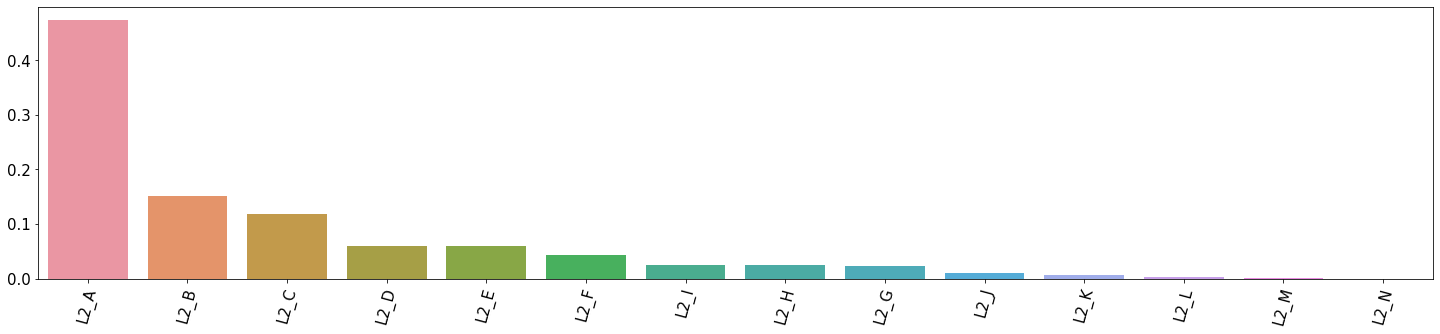
\includegraphics[width=1\textwidth]{./Figures/cap3-distribucion.png}
	\caption{Proporción de casos.}
	\label{fig:cap3-distribucion}
\end{figure}

También se realizó un análisis de las longitudes de los textos. En promedio, la cantidad de palabras en los mensajes fue de 78 previo a aplicar preprocesamiento, 71 aplicando una parte (se dejan las \textit{stopwords}) y 44 cuando se aplicó el preprocesamiento completo.

En la figura \ref{fig:cap3-longitudes} podemos observar la longitud promedio para cada categoría. En cada barra se puede ver la longitud del texto sin preprocesamiento, con preprocesamiento dejando \textit{stopwords} y también removiéndolas. Hay dos categorías cuya longitud promedio es particularmente elevada.

\begin{figure}[htbp]
	\centering
	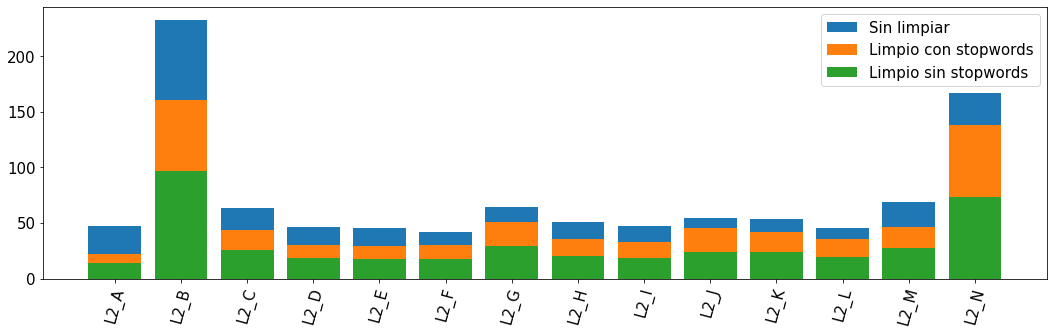
\includegraphics[width=1\textwidth]{./Figures/cap3-longitudes.png}
	\caption{Longitud de los mensajes.}
	\label{fig:cap3-longitudes}
\end{figure}

\subsection{Integración de los modelos}

A continuación se presenta la figura \ref{fig:cap3-redes} dónde se puede ver cómo fue concebida la arquitectura de la solución de los modelos de IA.

Se tiene un clasificador que en primera instancia hace la predicción de las categorías de primer nivel, y luego se tienen clasificadores para cada subcategoría de segundo nivel. Esto significa que en total se entrenaron 15 modelos: el general y 14 de subcategorías.

\begin{figure}[htbp]
	\centering
	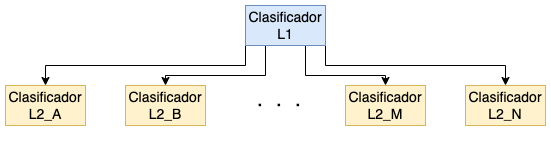
\includegraphics[width=.8\textwidth]{./Figures/cap3-redes.png}
	\caption{Diagrama general de los modelos de IA.}
	\label{fig:cap3-redes}
\end{figure}

Este diseño presenta una serie de ventajas, entre las que principalmente se destaca su diseño modular. Esto es importante para la etapa de soporte a futuro, ya que si surge una nueva categoría o se quiere mejorar una parte de la clasificación, sólo es necesario trabajar en el modelo afectado dejando los demás intactos.

Además, al hacer que cada clasificador tenga que realizar una tarea más específica, su \textit{head} de clasificación también queda más simple.

\subsection{Entrenamiento de los modelos base}

Un modelo base o \textit{baseline} es un modelo simple que actúa como referencia y sirve para tener con qué comparar cuando se entrenan modelos más complejos. 

Las ventajas de utilizar un modelo base son las siguientes \citep{WEBSITE:23}:
\begin{itemize}
	\item Se entrenan rápidamente y sin recursos especializados.
	\item Permite tener un mejor entendimiento en etapas tempranas.
	\item Sirven para encontrar errores y poner a prueba suposiciones.
	\item Sirven para medir el progreso de los modelos más complejos.
\end{itemize}

Como se mencionó en el capítulo \ref{Chapter2}, para este trabajo el \textit{baseline} elegido fue CNB de la librería Scikit-Learn. La clase provista se llama \textit{ComplementNB} y provee un método \textit{fit} para realizar el entrenamiento y un método \textit{predict} para realizar una predicción sobre datos que se pasan como parámetro.

El entorno donde se realizó el entrenamiento fue una computadora local.

\subsubsection{Modelos base en validación cruzada}

Hubo algunas categorías en particular que cuando se quiso entrenar el clasificador L2, contaban con muy pocos datos incluso tomando del año 2023. Estas categorías fueron:
\begin{itemize}
	\item L2\_L.
	\item L2\_N.
\end{itemize}

La primera contaba con un total de 200 casos y cuando se incluyeron los de 2023  se llegó a tener 267. Para este caso, lo que se hizo fue obtener una métrica en validación cruzada usando la clase RepeatedStratifiedKFold de Scikit-Learn con 5 \textit{folds} y 5 repeats. Luego se procedió a entrenar el modelo CNB final utilizando el set de datos completo.

La segunda contaba originalmente con sólo 2 casos y cuando se incluyeron los de 2023 se llegó a 8. Este resultó ser un caso muy extremo, donde se utilizó otra técnica de validación cruzada con la clase LeaveOneOut de Scikit-Learn. Lo que hace esta técnica es ir apartando un dato por \textit{fold} y entrenar con el resto. Una vez tomada la métrica, se entrenó el CNB final con todos los datos.

\subsection{Entrenamiento de BERT}

Como los textos del \textit{dataset} estaban escritos en español, se utilizó la red BETO. Este modelo es un modelo BERT entrenado con el dataset \textit{spanish unannotated corpora} que cuenta con casi tres millardos de palabras. Está disponible dentro de la librería Transformers de HuggingFace para Python, tanto en Pytorch como en Tensorflow. Para este trabajo se utilizó esta última.

Por otro lado, estos modelos pre-entrenados deben ser adaptados para realizar tareas como clasificación de texto. En la figura \ref{fig:cap3-downstream} se muestra un esquema de entrenamiento de BETO.

\begin{figure}[htbp]
	\centering
	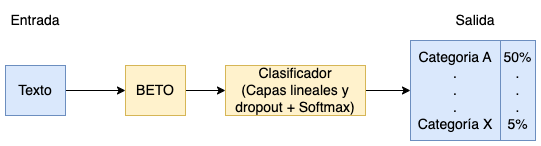
\includegraphics[width=.9\textwidth]{./Figures/cap3-downstream.png}
	\caption{Esquema de entrenamiento de BERT para clasificación de texto.}
	\label{fig:cap3-downstream}
\end{figure}

Se puede notar que sobre el modelo pre-entrenado de BETO se agrega: un \textit{head} de clasificación compuesto por perceptrones multicapa combinados con técnicas de regularización como \textit{dropout} y por último \textit{softmax} como función de activación para realizar la tarea de clasificación per se.

\subsubsection{Aprendizaje por transferencia}
\label{section:tf}

El aprendizaje por transferencia consiste en entrenar un modelo en un conjunto de datos a gran escala y luego usar ese modelo previamente entrenado para llevar a cabo el aprendizaje para otra tarea posterior (la tarea objetivo) \citep{WEBSITE:24}.

Se distinguen tres métodos para transferir el aprendizaje:
\begin{itemize}
	\item Extracción de características: se usan las capas pre-entrenadas para extraer características o \textit{features} de los datos. Los pesos de las capas inferiores no se actualizan durante el \textit{backpropagation}.
	\item Ajuste fino: se ajustan todos los parámetros del modelo.
	\item Extracción de capas: se extraen sólo las capas necesarias para la tarea en cuestión.
\end{itemize}

Para este trabajo, el aprendizaje por transferencia consistió en utilizar el modelo pre-entrenado de BETO y luego ajustarlo para la tarea de clasificación de reclamos.

En primera instancia se utilizó el método de extracción de características que consistió en congelar las capas de BETO y dejar libre el \textit{head} de clasificación para entrenar sus pesos. Para esto, se dejó el \textit{learning rate} default de Tensorflow.

\begin{figure}[htbp]
	\centering
	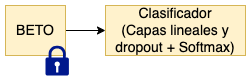
\includegraphics[width=.4\textwidth]{./Figures/cap3-feature-extraction.png}
	\caption{Técnica de extracción de características.}
	\label{fig:cap3-feature-extraction}
\end{figure}

Luego, se realizó un ajuste fino, dejando libres todas las capas del modelo para ajustar todos sus pesos, esta vez con un \textit{learning rate} más bajo.

\begin{figure}[htbp]
	\centering
	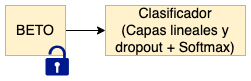
\includegraphics[width=.4\textwidth]{./Figures/cap3-fine-tuning.png}
	\caption{Técnica de ajuste fino.}
	\label{fig:cap3-fine-tuning}
\end{figure}

La técnica de extracción de capas no fue utilizada en este trabajo.

\subsubsection{Entorno de entrenamiento}

Como se menciona en el capítulo \ref{Chapter2}, para entrenar a BETO se utilizó un entorno de trabajo en la nube llamado Vertex AI Workbench. Se diferencian dos tipos de instancias:
\begin{itemize}
	\item Los \textit{notebooks} administrados: son entornos administrados por Google.
	\item Los \textit{notebooks} administrados por el usuario: permiten una mayor personalización y son ideales cuando se necesita mayor control sobre el entorno.
\end{itemize}

La instancia utilizada fue la segunda: las administradas por el usuario. El \textit{hardware} con el que contaba era el siguiente:
\begin{table}[h]
	\centering
	\caption[Especificaciones técnicas Vertex]{Especificaciones técnicas del entorno de entrenamiento.}
	\begin{tabular}{l c}    
		\toprule
		\textbf{Componente}			& 			\textbf{Descripción}  \\
		\midrule	
		Versión del ambiente		& 			M107  \\
		Tipo de máquina 			& 			n1-standard-8  \\
		Versión de CPU				&			Intel Xeon E5 \\
		Nro. de núcleos virtuales 	& 			8 vCPUs \\
		Memoria RAM 				& 			30 GB  \\
		Nro. de placas de video 	& 			1  \\
		Versión de placa de video 	& 			NVIDIA T4 \\
		Memoria de placa de video	& 			16 GB GDDR6  \\
		Almacenamiento				&			1 HDD x 200 GB \\
		\bottomrule
		\hline
	\end{tabular}
	\label{tab:vertex}
\end{table}

Por otro lado, se decidió utilizar el entorno TensorFlow Enterprise 2.11 como imagen virtual de la instancia, lo que permitió tener todos los \textit{drivers} de la placa de video pre-instalados y además contaba con el sistema de paquetes Conda con las librerías de TensorFlow para Python también pre-instaladas. Tener esa configuración cubierta por la nube de Google resultó en una gran ventaja porque evitó el tener que analizar la compatibilidad entre el \textit{hardware} y el \textit{software}.

\subsubsection{Puntos de control}

Para evitar pérdida de información accidental en la etapa de entrenamiento se utilizó una clase de TensorFlow que se llama ModelCheckpoint.

ModelCheckpoint es un \textit{callback} que, dependiendo de como se configure, puede ejecutarse al finalizar una época o cada cierta cantidad de lotes o \textit{batches}. Su función principal es guardar los pesos de la red y el estado del optimizador al almacenamiento permanente para no perder esa información en caso de que se apague la instancia o surja algún error. Se pueden configurar criterios de guardado como, por ejemplo, sólo si mejoró una métrica o la función de pérdida.

La configuración usada fue:
\begin{table}[h]
	\centering
	\caption[Configuración ModelCheckpoint]{Configuración del ModelCheckpoint.}
	\begin{tabular}{l c}    
		\toprule
		\textbf{Parámetro}			& 			\textbf{Valor}  \\
		\midrule	
		Nombre del archivo			& 			Nombre del archivo en extensión h5  \\
		Métrica a monitorear 		& 			Pérdida para lote de entrenamiento  \\
		Guardar sólo el mejor		&			Sí \\
		Modo de la métrica 			& 			Minimizar \\
		Frecuencia de guardado 		& 			En cada época  \\
		\bottomrule
		\hline
	\end{tabular}
	\label{tab:checkpoint}
\end{table}

\subsubsection{Parada temprana}

Otro de los mecanismos de prevención de sobreajuste o \textit{overfitting} utilizados fue la parada temprana o \textit{early stopping}. La idea detrás de esta técnica es detener el entrenamiento cuando el modelo empieza a disminuir su capacidad de generalización.

Esto se puede notar en la imagen \ref{fig:cap3-overfitting} donde la función de pérdida para el lote de entrenamiento continúa disminuyendo pero para el lote de validación no.

\begin{figure}[htbp]
	\centering
	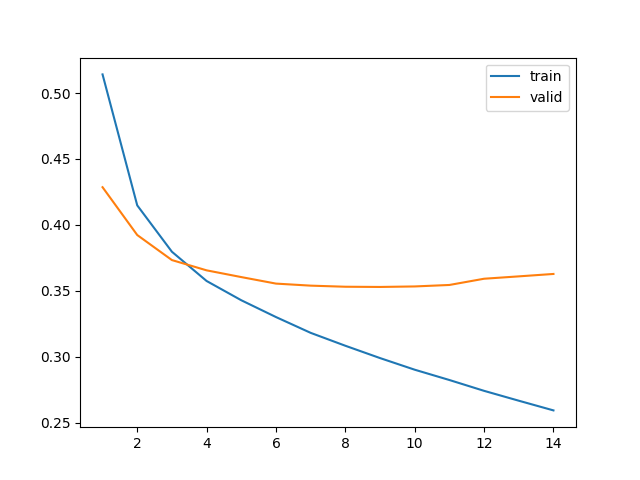
\includegraphics[width=.8\textwidth]{./Figures/cap3-overfitting.png}
	\caption{Funciones de pérdida a través de las épocas.}
	\label{fig:cap3-overfitting}
\end{figure}

La clase de TensorFlow utilizada para esto fue EarlyStopping. También es un \textit{callback} pero este lo que hace es ir monitoreando una métrica que se pasa como parámetro y luego de un par de épocas en las que no mejora o empeora, detiene el entrenamiento.

La configuración utilizada fue la siguiente:
\begin{table}[h]
	\centering
	\caption[Configuración EarlyStopping]{Configuración de EarlyStopping.}
	\begin{tabular}{l c}    
		\toprule
		\textbf{Parámetro}			& 			\textbf{Valor}  \\
		\midrule
		Métrica a monitorear		& 			Pérdida para lote de validación  \\
		Delta mínimo				& 			0 \\
		Paciencia					& 			5 épocas  \\
		Verboso						& 			Sí  \\
		Modo						& 			Automático  \\	
		Restaurar mejores pesos 	& 			Sí  \\
		Comienzo					& 			Época 0  \\	
		\bottomrule
		\hline
	\end{tabular}
	\label{tab:earlystopping}
\end{table}

\subsubsection{Variaciones en el entrenamiento}

Al momento de realizar los distintos entrenamientos de BETO, se analizaron qué variaciones se podían realizar en sus etapas desde el preprocesamiento hasta el entrenamiento per se, con el objetivo de intentar maximizar el desempeño del modelo. 

Una de esas variaciones fue dejar o remover las \textit{stopwords}. Esto se puede ver en la imagen \ref{fig:pipeline-texto} donde el paso de ``Remoción de \textit{stopwords}'' aparece en líneas punteadas. Por la forma en que los modelos de BERT aprenden del contexto, en todos los resultados el desempeño mejoró al dejarlas.

Otra variación que se intentó probar fue cambiar el largo de la secuencia. Los modelos de BERT admiten hasta un máximo de 512 \textit{tokens}. El desafío aquí es que a mayor largo de secuencia, habrá mayor consumo de memoria, y la placa de video utilizada estaba limitada en 16 GB. Otra consecuencia es que al consumir más memoria, obliga a reducir el \textit{batch size}.

Para la primer parte del entrenamiento, donde las capas inferiores estaban bloqueadas se utilizó un largo de secuencia de 128 con el tamaño del \textit{batch} en 128 muestras.

Para la segunda parte del entrenamiento, donde se realizó un ajuste fino a todas las capas de la red, se utilizó también un largo de secuencia de 128 pero en este caso hubo que reducir el tamaño del \textit{batch} a 24 muestras.

Cuando recién se estaban arrancando con los entrenamientos, se probó utilizar un largo de secuencia de 512 y con un \textit{batch} de 8, pero estas pruebas fueron desestimadas porque no había mejoras significativas en el desempeño y el entrenamiento demandaba mucho tiempo.

\subsubsection{Técnicas para el desbalance de clases}

La distribución de categorías presentaban un desbalance por la naturaleza misma de los reclamos. Hay reclamos con mayor probabilidad de ocurrencia que otros, ya sea porque una funcionalidad se utiliza más, porque tiene mayor propensión a fallar o simplemente porque genera más consultas por parte de los usuarios.

Entre los métodos disponibles para tratar el desbalance había \citep{ARTICLE:7} \citep{WEBSITE:25}:
\begin{itemize}
	\item Reagrupar categorías minoritarias en una sola.
	\item Sobremuestreo aleatorio: consiste en repetir casos de las clases minoritarias de forma aleatoria.
	\item Submuestreo aleatorio: consiste en eliminar casos de las clases mayoritarias de forma aleatoria.
	\item \textit{Text augmentation}: consiste en realizar manipulaciones sobre los textos originales como, por ejemplo, reemplazar palabras por sus sinónimos de forma aleatoria, para generar nuevos casos de las clases minoritarias.
	\item \textit{Hidden space augmentation}: consiste en generar nuevos vectores en el espacio de representación de BERT reemplazando partes pequeñas de un vector con otras de otro vector de la misma clase.
	\item Pesos para las clases: consiste en modificar la función de pérdida de la red a través del uso de un vector con pesos ponderados para cada clase, dándole mayor importancia a las clases minoritarias.
\end{itemize}

La primera opción de reagrupar categorías fue descartada porque el área de atención al cliente tiene categorías de reclamo pre-definidas que no se pueden modificar.

La opción de sobremuestreo podía generar sobreajuste por lo que fue descartada. Por otro lado, la opción de submuestreo también fue descartada porque implicaba pérdida de información importante para los reclamos que tienen mayor probabilidad de ocurrencia, y que en definitiva son los que suelen tratar más a menudo en el área.

Las opciones de \textit{augmentation} no llegaron a probarse por su complejidad y tiempo adicional que llevaría en el desarrollo. Sin embargo, pueden ser una gran alternativa para probar en caso de que se quiera seguir evolucionando el modelo a futuro.

Para este trabajo, se decidió probar \textit{class weights} o pesos para las clases utilizando la clase class\_weight de Scikit-Learn para generar el vector de pesos y luego pasándolo como parámetro a TensorFlow en la etapa de entrenamiento.

\subsubsection{Optimizadores}

Inicialmente, en los entrenamientos realizados se utilizó el optimizador Adam, que es el que viene por defecto en la librería de TensorFlow. De hecho, cuando fue lanzado BERT, sus autores mencionan que \citep{ARTICLE:8}:
\begin{itemize}
	\item Utilizaron el optimizador Adam con un \textit{batch size} de 256, un \textit{learning rate} de 1e-4 y 40 épocas para el pre-entrenamiento.
	\item Utilizaron el optimizador Adam con un \textit{batch size} de 16 o 32, un \textit{learning rate} de 5e-5, 3e-5 o 2e-5 y un número de épocas de entre 2 y 4 para realizar el ajuste fino.
\end{itemize}

Sin embargo, diversos artículos mencionan que utilizar el optimizador LAMB \textit{(Layer-wise adaptive moments optimizer for batch training)} tiene un mejor desempeño en pruebas, una mejor capacidad de generalización y además permite entrenar con \textit{batches} de mayor tamaño y \textit{learning rates} más grandes, por lo que también se decidió probar con este optimizador para los entrenamientos \citep{ARTICLE:9} \citep{WEBSITE:26}.

El algoritmo está basado en Adam, por lo que es muy similar a este. La principal diferencia es que calcula una relación conocida como ``factor de confianza'' que sirve para normalizar los gradientes y evitar divergencias. Esta normalización es doble: (i) normaliza por dimensión con respecto a la raíz cuadrada del segundo momento utilizado en Adam y (ii) normaliza por capas.

En la figura \ref{fig:cap3-lamb} se puede observar los valores de la función de pérdida y el nivel exactitud en pruebas para Adam (en azul) y LAMB (en rojo) a través del tiempo en el conjunto de datos MNIST.

\begin{figure}[htbp]
	\centering
	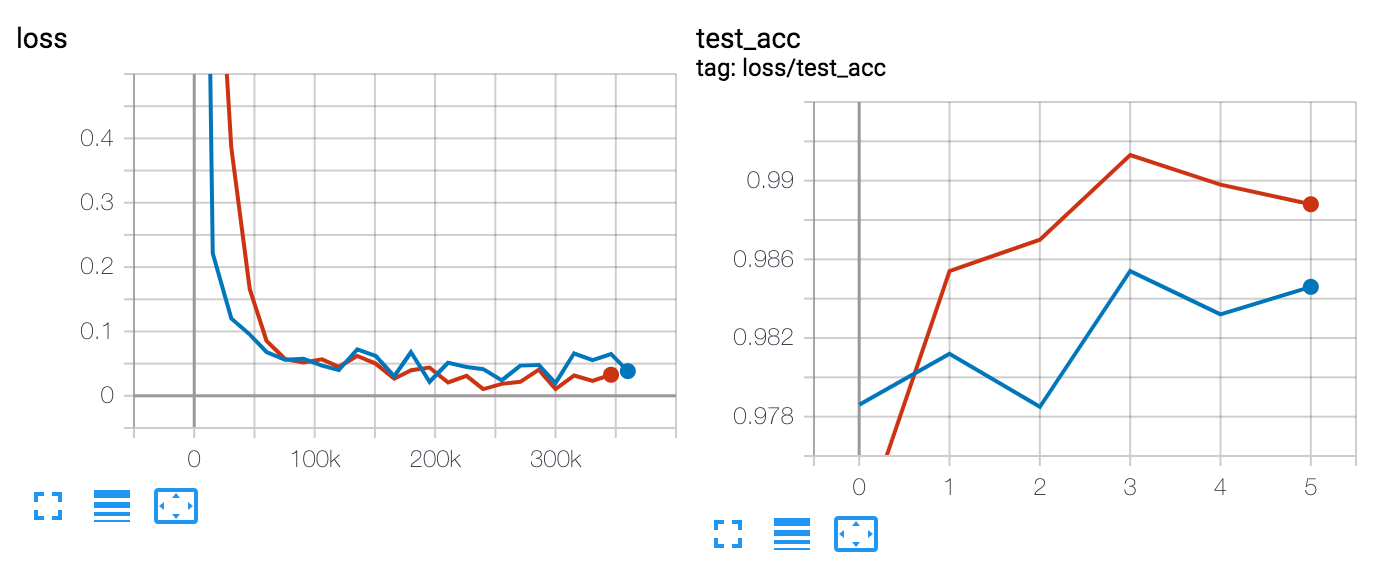
\includegraphics[width=.8\textwidth]{./Figures/cap3-adam-vs-lamb.png}
	\caption{Función de pérdida y exactitud para Adam (azul) y LAMB (rojo) para MNIST\protect\footnotemark.}
	\label{fig:cap3-lamb}
\end{figure}

\footnotetext{Imagen tomada de \url{https://towardsdatascience.com/an-intuitive-understanding-of-the-lamb-optimizer-46f8c0ae4866}}

\section{Empaquetamiento del código y artefactos}

Para empaquetar el código se utilizó la herramienta Docker en conjunto con un GitHub Workflow desarrollado en el mismo repositorio. Los pasos realizados fueron los siguientes:
\begin{enumerate}
	\item Escribir los archivos de código que hacen la predicción.
	\item Escribir un archivo con las librerías de Python necesarias.
	\item Escribir el GitHub Workflow para generar una imagen de Docker y cargarla al Artifact Registry.
	\item Cargar las credenciales de la nube de Google como \textit{secret} en el repositorio.
	\item Escribir el Dockerfile.
	\item Ejecutar el Workflow y verificar la creación de la imagen en el Artifact Registry.
\end{enumerate}

A continuación, en la figura \ref{fig:cap3-docker-integracion} se puede ver la integración de los distintos componentes para generar una imagen de Docker.

\begin{figure}[htbp]
	\centering
	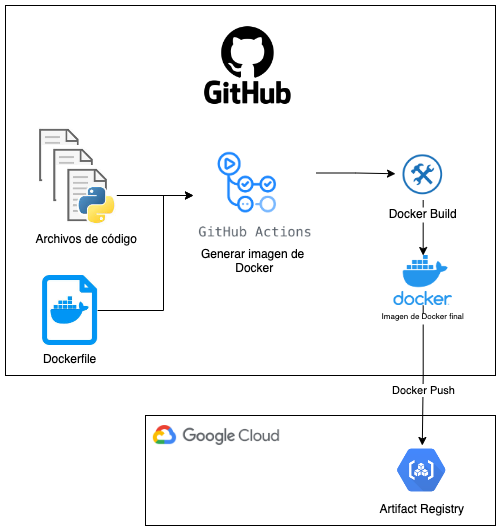
\includegraphics[width=.6\textwidth]{./Figures/cap3-docker-integracion.png}
	\caption{Interacción de los distintos componentes.}
	\label{fig:cap3-docker-integracion}
\end{figure}

En el repositorio de GitHub se encuentran los archivos de código y el Dockerfile. Además dentro del mismo repositorio se encuentra un archivo ``.yaml'' que describe un GitHub Workflow. Este archivo contiene una secuencia de pasos (los GitHub Actions) que deben ejecutarse para generar una imagen de Docker. Estos Actions son ejecutados por un GitHub Runner, que son máquinas virtuales hospedadas por la plataforma. Entre otras cosas, se ejecutan Actions para clonar el código en el Runner, autenticarlo contra la nube de Google, configurar Docker para conectarse al Artifact Registry y comenzar el proceso de construcción.

En la figura \ref{fig:cap3-gh-docker} puede verse el menú de GitHub desde donde ejecutar el flujo manualmente para generar la imagen de Docker.

\begin{figure}[htbp]
	\centering
	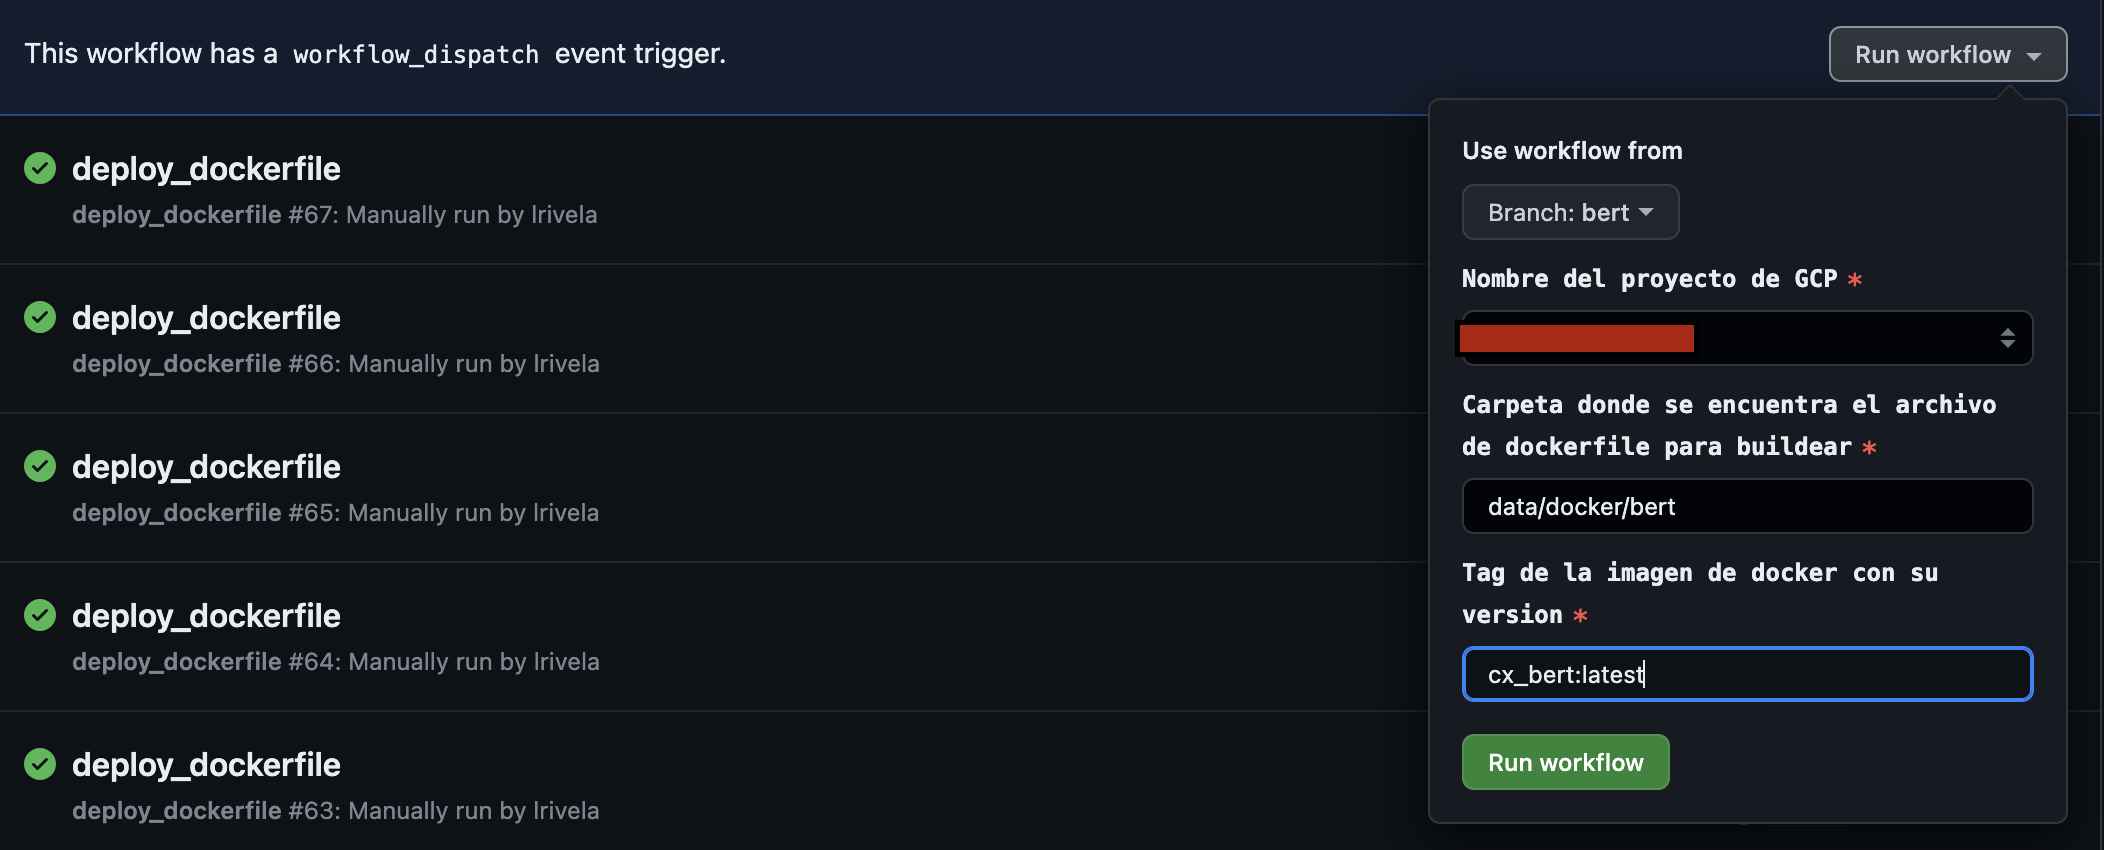
\includegraphics[width=.8\textwidth]{./Figures/cap3-gh-docker.png}
	\caption{Menú de GitHub para ejecutar el flujo de trabajo.}
	\label{fig:cap3-gh-docker}
\end{figure}

El Dockerfile es un archivo que incluye instrucciones para crear una imagen de Docker. En la figura \ref{fig:cap3-docker-dockerfile} puede verse en detalle.

\begin{figure}[htbp]
	\centering
	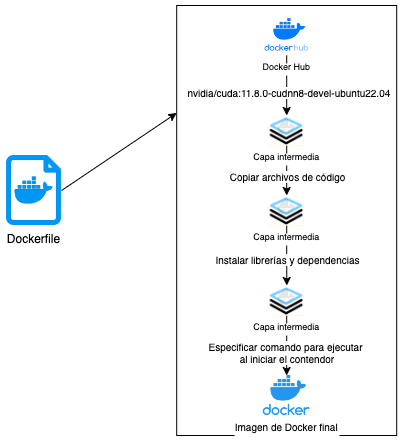
\includegraphics[width=.6\textwidth]{./Figures/cap3-docker-dockerfile.png}
	\caption{Vista detallada de un Dockerfile.}
	\label{fig:cap3-docker-dockerfile}
\end{figure}

Este archivo debe comenzar con una sentencia ``\textit{FROM}'' que indica la imagen padre desde la cual se va a crear la imagen. Para este trabajo se utilizó una imagen de la empresa Nvidia que está basada en el sistema operativo Ubuntu y que incluye todos los \textit{drivers} necesarios para utilizar una placa de video. La imagen se encuentra alojada en un repositorio público llamado Docker Hub.

Con el comando ``\textit{WORKDIR}'' se configura el directorio de trabajo dentro de la imagen de Docker y luego con el comando ``\textit{COPY}'' se le agregan los archivos Python y SQL del repositorio.

Con la ayuda del comando ``\textit{RUN}'' se instalan paquetes de Linux, el intérprete de Python y sus dependencias. Por último se especifica el comando a ejecutar para iniciar el contenedor de Docker con la sentencia ``\textit{CMD}''.


\section{Desarrollo del \textit{pipeline} de predicción}

En esta sección se describe cómo se ejecuta el código en la nube de Google para generar las predicciones del modelo y su posterior almacenamiento en una base de datos.

\subsection{Creación y ejecución del flujo de trabajo}

La herramienta seleccionada para dirigir la ejecución de código fue Apache Airflow, que en su versión administrada por la nube de Google se llama Cloud Composer.

En la figura \ref{fig:cap3-pipeline} puede verse cómo es el flujo para cargar un DAG a Airflow, desde su creación en el repositorio de código hasta su ejecución en un Pod de Kubernetes.

\begin{figure}[htbp]
	\centering
	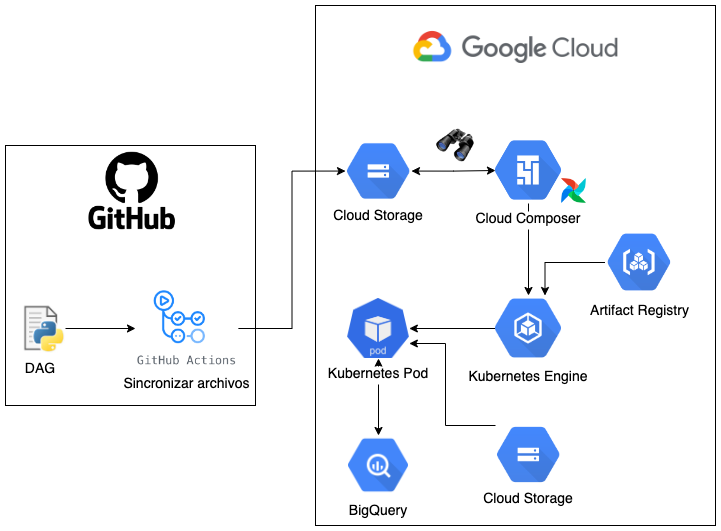
\includegraphics[width=.8\textwidth]{./Figures/cap3-pipeline.png}
	\caption{Interacción de los componentes del \textit{pipeline}.}
	\label{fig:cap3-pipeline}
\end{figure}

El proceso arranca generando un DAG en el repositorio dedicado para Airflow, que tiene un GitHub Workflow que sincroniza el archivo contra un contenedor de Cloud Storage llamado \textit{bucket}. 

El Cloud Composer está continuamente monitoreando si se cargaron nuevos archivos al \textit{bucket} que tiene configurado, y cuando así sucede, los carga en la base de Airflow. Luego lo procede a mostrar en su portal \textit{web}.

Un DAG puede ser programado para ejecutarse a intervalos regulares de tiempo o también puede ser ejecutado manualmente. Cuando se ejecuta, se comienzan a ejecutar distintos operadores en su flujo de trabajo. En la figura \ref{} puede verse la estructura del DAG desarrollado.

[FIGURA DAG]

Todos los operadores que componen este DAG son del tipo GKEStartPodOperator. Este operador hace que Airflow se conecte con el motor de Kubernetes Engine que se pase como parámetro e instancia un Pod. Las configuraciones más importantes que se utilizaron fueron:
\begin{itemize}
	\item El nombre del \textit{cluster} de GKE donde se va a instanciar el Pod.
	\item La localización del \textit{cluster} de GKE.
	\item La imagen de Docker que se generó en el Artifact Registry con el código.
	\item Variables de entorno que se le van a pasar al Pod: qué archivo de Python ejecutar, las tablas donde guardar información temporal, los \textit{datasets} de las tablas, el \textit{storage} donde están los archivos con los pesos de los modelos, etc.
	\item Los recursos del pod (CPU, RAM, Cantidad de placas de video).
	\item El nodo de Kubernetes donde asignar la ejecución del Pod para asegurar que tenga placa de video.
\end{itemize}

Al final del DAG se define el ruteo entre los operadores para definir como se conectan y cómo son las reglas de ejecución.

Los estados por los que pasa un Pod para instanciarse pueden verse en la figura \ref{fig:cap3-pod-lc}.

\begin{figure}[htbp]
	\centering
	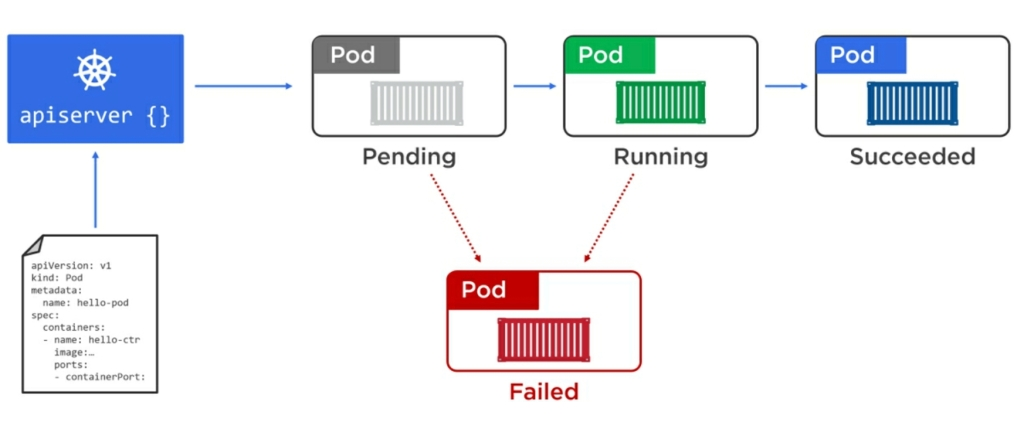
\includegraphics[width=.8\textwidth]{./Figures/pod-lifecycle.jpeg}
	\caption{Estados del ciclo de vida de un Pod de Kubernetes\protect\footnotemark.}
	\label{fig:cap3-pod-lc}
\end{figure}

\footnotetext{Imagen tomada de \url{https://sunitc.dev/2020/12/26/kubernetes-pods/}}

A continuación se explica cada uno de ellos \citep{WEBSITE:27}:
\begin{itemize}
	\item \textit{Pending}: Cuando el Pod ha sido aceptado por el \textit{cluster} de Kubernetes, pero los contenedores aún no están listos. Por ejemplo, la imagen de Docker aún se está descargando.
	\item \textit{Running}: Cuando el Pod ha sido asignado a un nodo de Kubernetes y tiene su contenedor corriendo.
	\item \textit{Succeeded}: Cuando el contenedor del Pod ha terminado exitosamente. Por ejemplo, finalizó la ejecución del código de Python.
	\item \textit{Failed}: Cuando el contenedor termina con un error. Por ejemplo, un error de programación en el código o un error en la configuración de Kubernetes.
\end{itemize}

\subsection{Parametrización de los contenedores}


